\documentclass{beamer}
%
% Choose how your presentation looks.
%
% For more themes, color themes and font themes, see:
% http://deic.uab.es/~iblanes/beamer_gallery/index_by_theme.html
%
\mode<presentation>
{
  \usetheme{default}      % or try Darmstadt, Madrid, Warsaw, ...
  \usecolortheme{default} % or try albatross, beaver, crane, ...
  \usefonttheme{default}  % or try serif, structurebold, ...
  \setbeamertemplate{navigation symbols}{}
  \setbeamertemplate{caption}[numbered]
  %\setbeamertemplate{footline}[frame number]
}
\usepackage{outlines}
 
\usepackage{graphicx}
\usepackage[english]{babel}
\usepackage[utf8x]{inputenc}
\title{Model Checking and Systems Verification (MCSV)}
\setbeamertemplate{footline}[frame number]
\author{Instructor; M.K. Srivas \\
TA: Zubin Duggal}

\begin{document}
\begin{frame}
  \titlepage
\end{frame}

% Uncomment these lines for an automatically generated outline.
%\begin{frame}{Outline}
%  \tableofcontents
%\end{frame}

\section{Outline}

\begin{frame}{Embedded Systems}
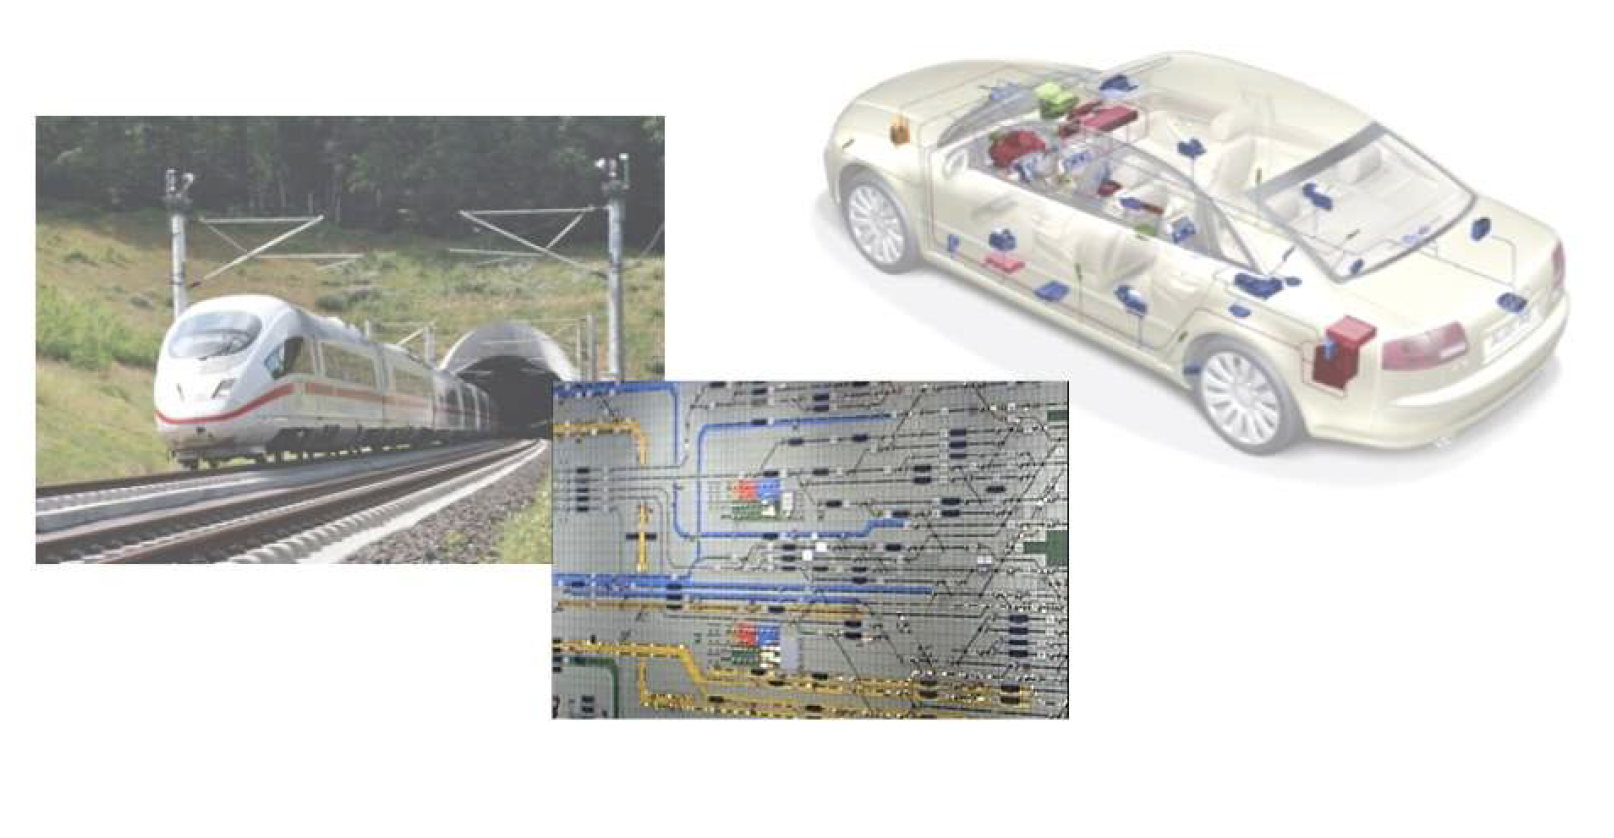
\includegraphics[scale=0.4]{pics/motivpic.png}
\begin{itemize}
\item Embedded (HW+SW+FW) systems are a complex parts of real life machines
\end{itemize}
\end{frame}

\begin{frame}{Model Checking: Motivation}
\begin{itemize}
\item <1-> Traditional methods: Simulation and testing
\begin{itemize}
\item <2-> Do not guarantee 100\% coverage
\item<3-> Expensive; Labour intensive and time consuming
\end{itemize}

\item<4->Can we have methods that guarantee 100\% coverage
\begin{itemize}
\item<5->Formal Verification: Methods based on Logic and Automata theory
\item<6-> Model Checking is one such popular technique
\end{itemize}
\end{itemize}
\end{frame}

\begin{frame}{Model Checking: Cited for Turing Award in 2007 \\
(Invented: 1986)}
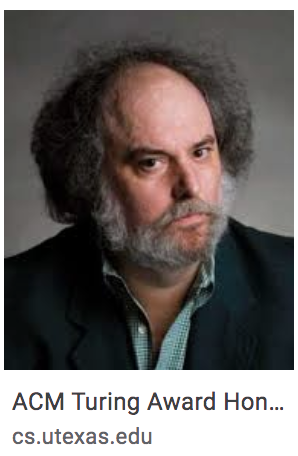
\includegraphics[scale=0.4]{pics/allen.png}\hfill
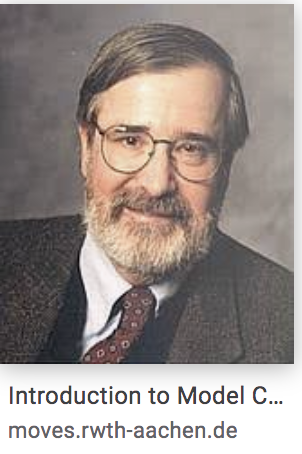
\includegraphics[scale=0.4]{pics/clarke.png}\hfill
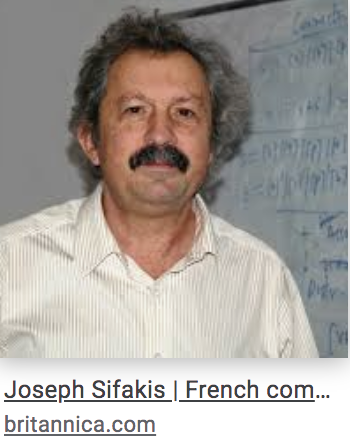
\includegraphics[scale=0.4]{pics/sifakis.png}

E. Allen Emerson~~~~~~~~~~~Edmund Clarke~~~~~~~~~~~~Joseph Sifakis
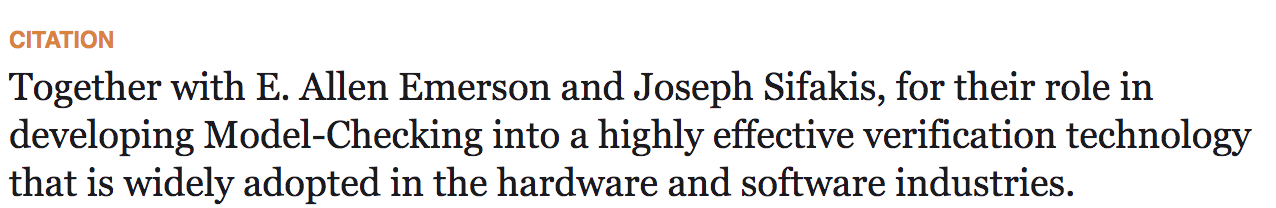
\includegraphics[scale=0.5]{pics/Citation.png} 
\end{frame}

\begin{frame}{What Kind of Systems and Properties?}
\uncover<1->{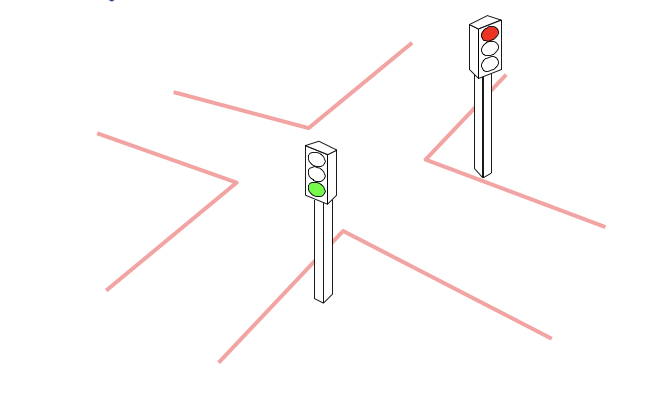
\includegraphics[scale=0.3]{pics/trafficsignal.png}}\hfill
\uncover<3->{\includegraphics[scale=0.2]{pics/mod3cnt.png}}\\
\uncover<2->{\tiny{``traffic lights should never be green at the same time''}} \hfill
\uncover<4->{\tiny{``the counter value (`ab') is always $\leq$ 3''}}
\vfill
\uncover<5->{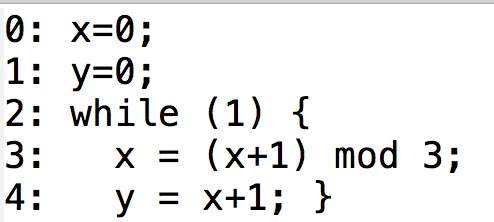
\includegraphics[scale=0.3]{pics/code.png}}\hfill
\uncover<7->{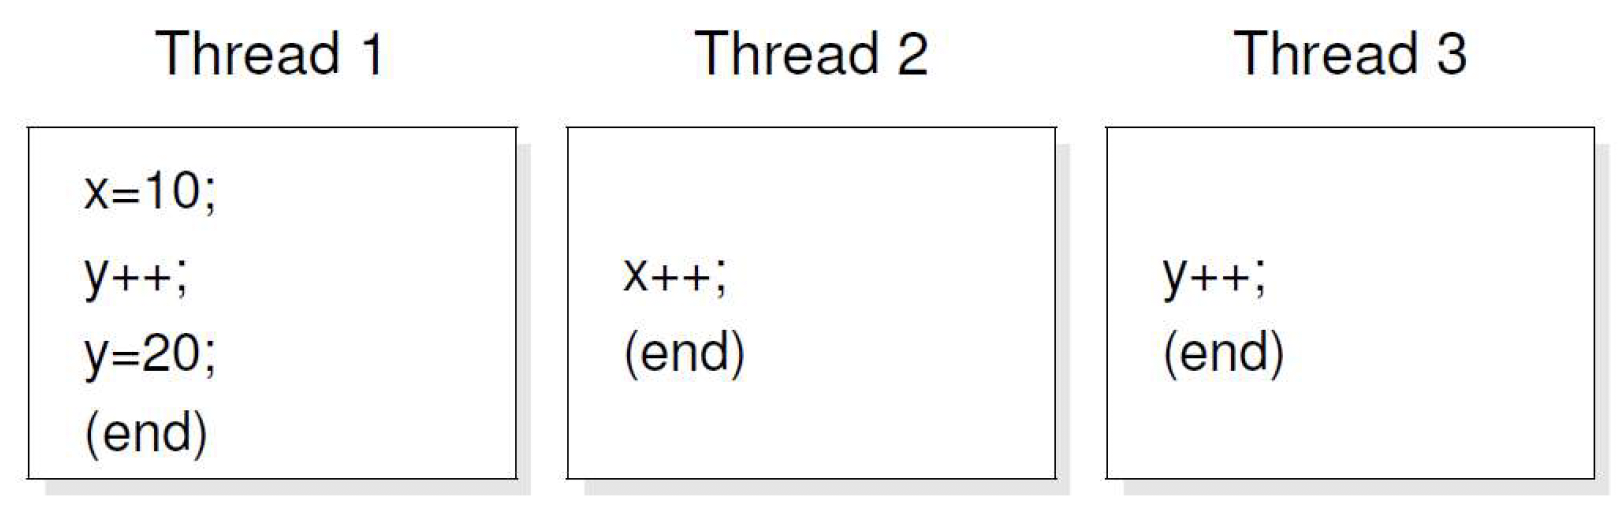
\includegraphics[scale=0.15]{pics/concprog.png}}\\
\uncover<6->{\tiny{``@line~3: $y \geq x$ $always$ holds''}} \hfill
\uncover<8->{\tiny{``the program has no data races''}} \\
\uncover<6->{\tiny{``@line~3: x=0 holds infinitely often''}}

\end{frame}

\begin{frame}{What Kind of Systems Not} 
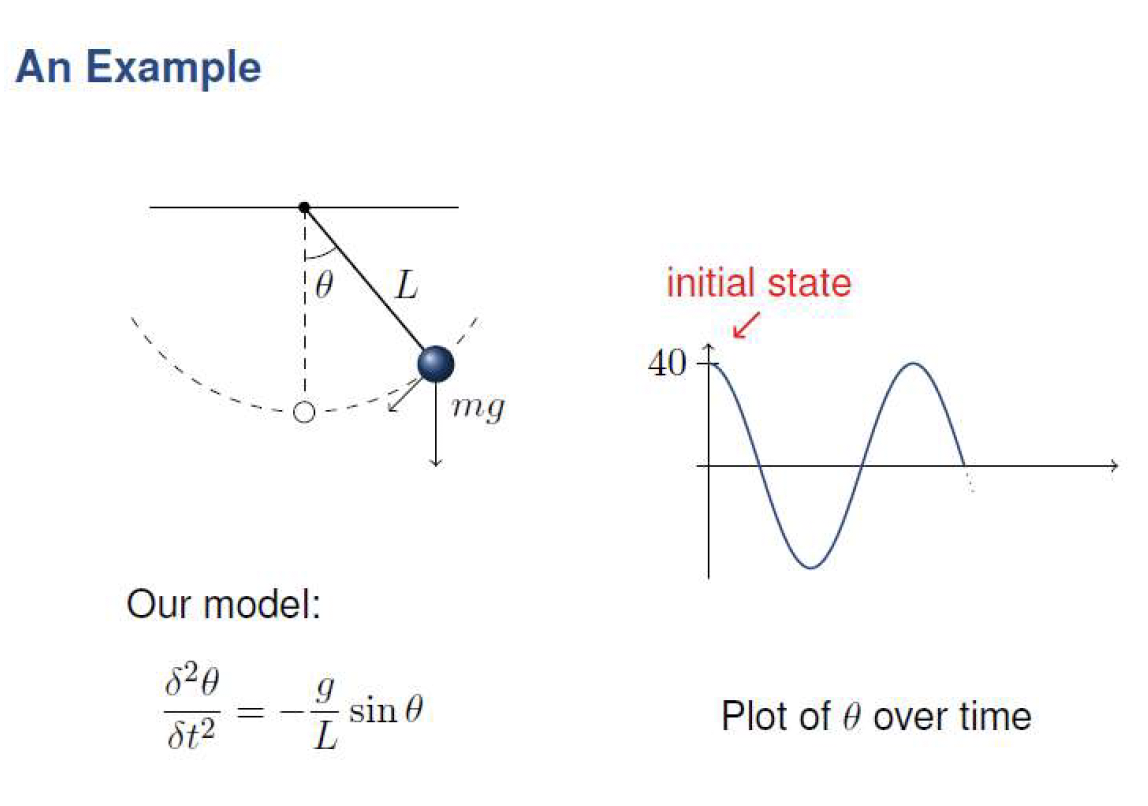
\includegraphics[scale=0.3]{pics/contdynamics.png}
\end{frame}

\begin{frame}{What do we need for formal verification?}
\begin{itemize}
\item<1-> Need a common formalism to model all systems of interest:
\textbf{Transition Systems (M)}

\item<2-> Need an expressive logic/language to specify desired properties \\
\textbf{``Special-purpose Temporal Logics (Prop)''}

\item<3-> Need efficient algorithms to automatically check properties \\
\textbf{M $\models$ Prop}
\end{itemize}
\end{frame}


\begin{frame}{Other Powerful Formal Verification Methods}
\begin{enumerate}
\item<1-> Abstract Interpretation (Static Analysis)
\begin{itemize}
\item Automatic, most scalable and widely used

\item Imprecise (False negatives)
\end{itemize}
\item<2-> Theorem Proving
\begin{itemize}
\item Most general: For Models and properties

\item Mostly Interactive
\end{itemize}

\item<3-> Model Checking
\begin{itemize}
\item Significant industry interest: Intel, ARM, MicrSoft, Google, Facebook
\item A very active research area
\end{itemize}
\end{enumerate}
\end{frame}

\begin{frame}{Brief Course Outline}
\begin{enumerate}
\item Modeling Systems (Kripke Structures)
\item Specifying Properties (Temporal logics: CTL, LTL, CTL*)
\item Verifying Properties (Model Checking for Temporal logics)
\item Tools Exercises: NuSMV, CBMC, SATABS
\item Abstraction and Induction: Scaling Techniques
\item Automata-Based Model Checking
\end{enumerate}
\end{frame}

\begin{frame}{Course Work and Grade Distribution}
\begin{enumerate}
\item  Written Assignments: 30\%
%\begin{enumerate}
%\item Modeling and Temporal Logic
%\item SAT and BDD Exerzises
%\end{enumerate}

\item  Tool Exercises: 30\%
%\begin{enumerate}
%\item Verification exercizes on tools NuSMV, CBMC, SAT-ABS
%\item 
%\end{enumerate}

\item  2 Quizzes: 40\%
\begin{itemize}
\item One can be a small programming project
\end{itemize}
\end{enumerate}
\end{frame}

\begin{frame}{Reference Text Book}
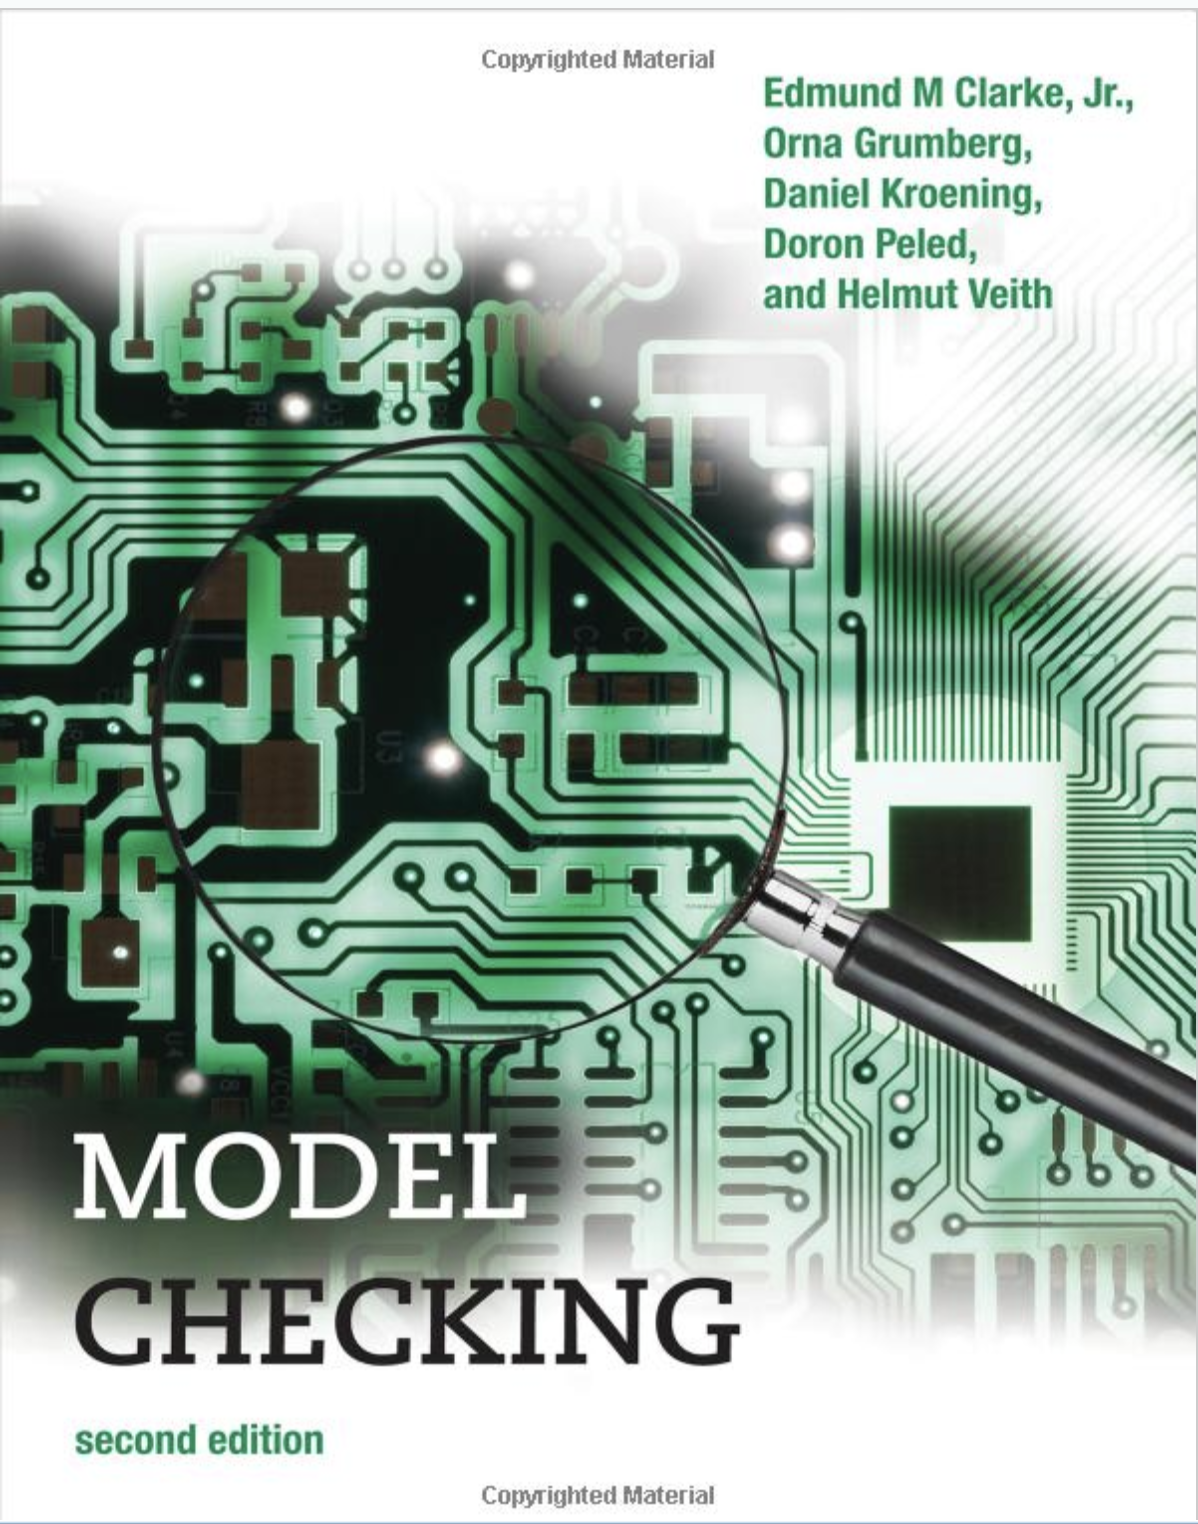
\includegraphics[scale=0.25]{pics/bookcover.png} \\
eTextBook will be made available for class \\
usage on shared (sign-up sheet) basis \\
Access details will be shared on Moodle
\end{frame}

\begin{frame}{Industry Recognition Anecdote}
\includegraphics[scale=0.25]{pics/billgates.png} 
\end{frame}

\begin{frame}{}
\begin{itemize}
\item 
\end{itemize}

\end{frame}



\begin{frame}{}

\end{frame}

\begin{frame}{}

\end{frame}

\end{document}
